\begin{figure}[t]
\centering
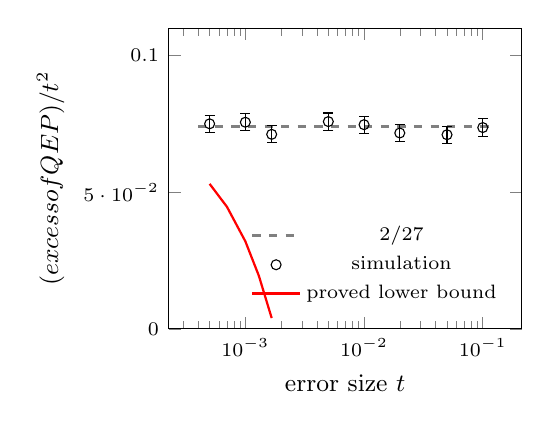
\begin{tikzpicture}
\begin{axis}[width=0.5\textwidth,height=5.4cm,xmode=log,xlabel={error size $t$},ylabel={$(\text{excess of QEP})/t^2$},ymin=0,ymax=0.11,
legend style={font=\scriptsize,at={(0.97,0.05)},anchor=south east,draw=none,fill=none},tick label style={font=\scriptsize},label style={font=\small}]
\addplot[gray,dashed,thick,domain=4e-4:0.12,samples=2] {2/27};
\addlegendentry{$2/27$}
\addplot[black,only marks,mark=o,mark size=1.8pt,error bars/.cd,y dir=both,y explicit] coordinates {(0.0005,0.0750302) +- (0,0.00315) (0.001,0.0756053) +- (0,0.00315) (0.00166667,0.0711813) +- (0,0.00315) (0.005,0.0758429) +- (0,0.00315) (0.01,0.0747112) +- (0,0.00314) (0.02,0.0716695) +- (0,0.00315) (0.05,0.0710288) +- (0,0.00315) (0.1,0.0736577) +- (0,0.00317)};
\addlegendentry{simulation}
\addplot[red,thick] coordinates {(0.0005,0.0530636) (0.0007,0.0446535) (0.001,0.0320321) (0.0013,0.0194031) (0.00166667,0.00395741)};
\addlegendentry{proved lower bound}
\end{axis}
\end{tikzpicture}\hfill
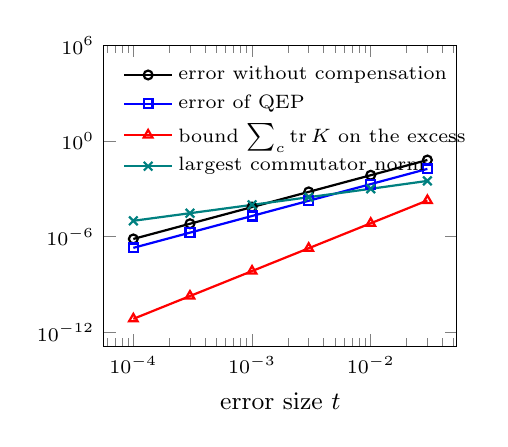
\begin{tikzpicture}
\begin{axis}[width=0.5\textwidth,height=5.4cm,xmode=log,ymode=log,xlabel={error size $t$},ymax=1e6,
legend style={font=\scriptsize,at={(0.03,0.97)},anchor=north west,draw=none,fill=none,legend cell align=left},tick label style={font=\scriptsize},label style={font=\small}]
\addplot[black,thick,mark=o,mark size=1.6pt] coordinates {(0.0001,7.2565e-07) (0.0003,6.53085e-06) (0.001,7.2565e-05) (0.003,0.000653088) (0.01,0.0072569) (0.03,0.0653409)};
\addlegendentry{error without compensation}
\addplot[blue,thick,mark=square,mark size=1.6pt] coordinates {(0.0001,2.0065e-07) (0.0003,1.80585e-06) (0.001,2.0065e-05) (0.003,0.000180588) (0.01,0.0020069) (0.03,0.0180911)};
\addlegendentry{error of QEP}
\addplot[red,thick,mark=triangle,mark size=1.8pt] coordinates {(0.0001,7.01033e-12) (0.0003,1.89279e-10) (0.001,7.01034e-09) (0.003,1.8928e-07) (0.01,7.01075e-06) (0.03,0.000189381)};
\addlegendentry{bound $\sum_c\mathrm{tr}\,K$ on the excess}
\addplot[teal,thick,mark=x,mark size=2.2pt] coordinates {(0.0001,1.0002e-05) (0.0003,3.0018e-05) (0.001,0.0001002) (0.003,0.000301811) (0.01,0.00102041) (0.03,0.00319144)};
\addlegendentry{largest commutator norm}
\end{axis}
\end{tikzpicture}
\caption{ReLU networks. Left: Example~\ref{ex:noflip}, rounding errors sampled from the uniform law of subtractive dither, $10^6$ independent runs per value of $t$, two standard errors; no activation changed state in any run. Right: the bottleneck family after Corollary~\ref{cor:hr} with $\eta=\tfrac1{10}$ and sign-valued errors, exact enumeration; here the correction helps, the bound on the excess decreases as $t^3$ and the commutator as $t$.}\label{fig:relu}
\end{figure}
